%\documentclass[11pt,a4paper,notitlepage]{article}
%\documentclass[11pt,a4,portrait,twocolumn,notitlepage,openright]{article}
%\documentclass[12pt,lETter,landscape,onecolumn,titlepage,openany]{report}
\documentclass[12pt,onecolumn,tightenlines,aps,amsmath,floatfix,notitlepage,nofootinbib]{revtex4}
\usepackage[T1]{fontenc}        % T1 fonts for output to postscript (looks better!)
\usepackage{palatino}           % For index at the end
\usepackage{amsmath}            % Advanced maths
\usepackage{amssymb}            % instead of \usepackage{latexsym}
%\usepackage{graphix}           % For graphics. PS. not included on socrates
\usepackage{graphicx}           % For pdflatex. Pictures must be in png, jpg, pdf format
%\usepackage{graphics}          % For latex. Pictures must be in eps, ps (ps needs bb)
\usepackage{pslatex}
\usepackage{epsfig}
\usepackage{epsf}
\usepackage[usenames]{color}
%\usepackage{braket}            % for Dirac Bra-Ket notation
\setlength{\unitlength}{1cm}
\pagestyle{plain}               % Alternatively, use empty(no header/footer), i
                                %   headings(no footer), myheadings
%\markright{head}               % If using \pagestyle{myheadings} need to specify this or \markboth
%\markboth{leftheading}{rightheading}

%\usepackage{fancyhrd}          % Fancy headers
%\pagestyle{fancy}
%\fancyhead{L,O}{\leftmark}     % Sets L (or R C) left heading
%\fancyfoot{R,E}{\rightmark}    % Sets R (or L C) right footer

\newcommand{\curl}{\nabla \times}
\newcommand{\diverg}{\nabla \cdot}
\newcommand{\V}[1]{\mathbf{#1}}
\newcommand{\bra}[1]{\langle #1|}
\newcommand{\ket}[1]{|#1\rangle}
\newcommand{\braket}[2]{\langle #1|#2\rangle}

% Page layout
%\setlength{\textwidth}{1em}     % Sets texwidth to the width of an "m"
%\setlength{\textheight}{1ex}    % Sets texheight to the height of an "x"
% Alternative units are cm,in,pt

%\setlength{\parindent}{2ex}
%\setlength{\parskip}{1ex plus 0.2ex minus 0.2ex}
%\renewcommand{\baselinestretch}{1.5}   % Sets spacing between lines to 150% of original.

%\pagenumbering{roman}          % sets numbering e.g. i,ii,iii. Alt use {Roman} for I,II,III
\pagenumbering{arabic}          % Sets numbering in arabic 
%\pagenumbering{alph}           % sets alphanumeric numbering or {Alph} for capitalisation

%\onecolumn                     % Formats pages in one columns
%\twocolumn                     % Formats pages in two columns

\begin{document}

\title{SAFiCF: A Simulated Annealing Fitting package for \\ Crystal Field inelastic neutron scattering data. \\ SAFiCF version 0.1 Manual}

\author{M. D. Le}
%\author{ucapmdl \and mdl27}    % One name after another
%\author{ucapmdl \\[1cm] mdl27}  % One name below another 
%\thanks{mdl acknowleges an epsrc studentship}

%\noaffiliation
\affiliation{London Centre for Nanotechnology, 17-19 Gordon St., London, WC1H 0AH}
\email{duc.le@ucl.ac.uk}

\date{\today}
%\date{20th August, 2004}

% The percent sign % denotes comments

%\begin{titlepage}
%Titlepage Text
%\end{titlepage}

%%% ----------------------------------------------------------------------

%\begin{abstract}

%\end{abstract}

\maketitle
%%% ----------------------------------------------------------------------

\tableofcontents                % Generates a table of contents

%%% ----------------------------------------------------------------------
%\newpage
\section{Acknowledgements} \label{sec-acknowledgements}

This package was first suggested by Prof. D. F. McMorrow, and also was also discussed at the LCN spin discussion group which gave many constructive suggestions. Thanks also to Andrew Walters for suggesting the Corana Simulated Annealing algorithm, and for the Fortran implementation of that algorithm on which this program is based. 

%%% ----------------------------------------------------------------------
\newpage
%\pagenumbering{arabic}         % Changes page numbering from here onwards
%\setcounter{page}{10}          % Resets page counter after, e.g., a \thispagestyle{}
%\pagebreak                     % Use this if using twocolumn

\section{Introduction} \label{sec-intro}

SAFiCF is a program for the Matlab environment that attempts to fit a set of crystal field parameters to inelastic neutron scattering (INS) data for \emph{rare earth} or \emph{localised actinide} compounds. It was written for Matlab 7 R14. It uses an implementation of the simulated annealing fitting algorithm due to Corana et. al.~\cite{CMMR87}. The block diagram for the program, labelling its constituent m-files is shown in figure~\ref{fg:block}. A brief theoretical description of crystal field excitations as observed in INS is given in section~\ref{sec-theory}, and the program itself is described in detail in section~\ref{sec-prog}, its usage in subsequent sections. 

\begin{figure}
  \begin{center}
    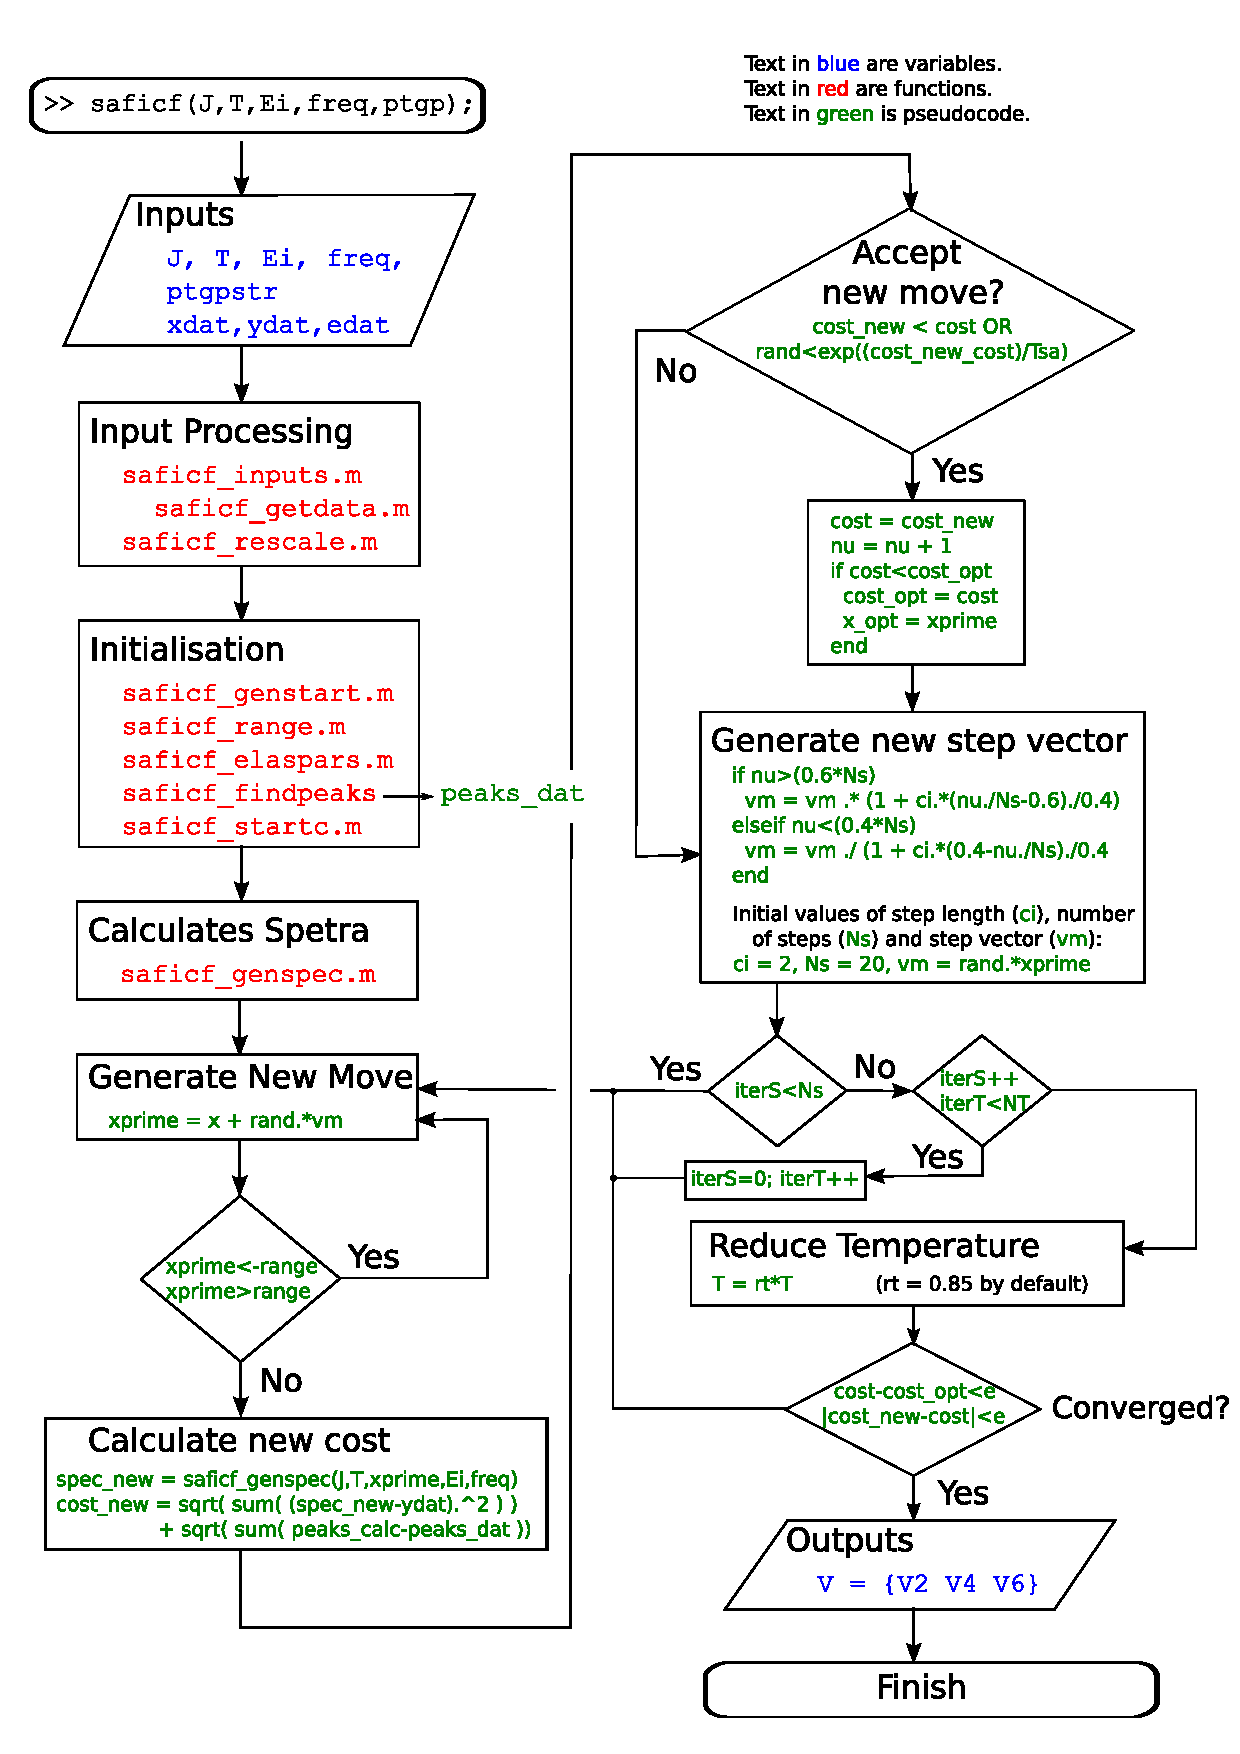
\includegraphics[width=\textwidth]{figs/block.pdf}
    \caption{\emph{Block diagram of the SAFiCF program}.} \label{fg:block}
  \end{center}
\end{figure}

%%% ----------------------------------------------------------------------

\section{Theoretical Background} \label{sec-theory}

Localised rare-earth and actinide ions are well described by $LS$-coupling with a ground state multiplet determined by Hund's Rules, and characterised by the total angular momentum quantum number $J$. In a free ion, these $J$-multiplets containing $2J+1$ levels labeled by $m_J = -J,\ldots,+J$ are degenerate. However, crystal field interactions arising from the breaking of the symmetry of free ions by the regular arrangements of a crystal will break this degeneract of the free ion $J$ multiplets. This occurs because whereas a free ion will have a Hamiltonian with spherical symmetry, the magnetic ions in a crystal will have a different site symmetry. 

Thus the effect of a crystal field can be thought of as a perturbation acting on free magnetic ions due to the mechanisms of crystal bonding. Initially it was attributed to the electric potential due to the charge distribution of surrounding ions on a magnetic ion within the crystal, hence the term \emph{crystalline electric field}. Expressing this contribution by a multipolar expansion centred on the magnetic ion yields ...

%Theory. 

%This involves equations.

%\begin{equation} \label{eq:landauer}
%G = \frac{e^2}{h} Tr(t^{\dagger}t)
%\end{equation}

%% \verb| is for verbatim mode, will print whatever is between the | |. 
%For non-numbered equations, miss out the \verb| \label{whatever} | bit, or use the short hand \verb| \[ eqn \] |:

%for fractions:
%\[ \frac{numerator}{denominator} \]

%% $ equation $ anything enclosed in dollar signs are equations
%use \verb|^| for superscript e.g. $F = \frac{GMm}{r^2}$
%use \verb|_| for subscript e.g. 2H$_2$ + O$_2$ = 2H$_2$O
%for sub or superscripts of more than one character, enclose in curly brackets: 

%\[  \delta_{mn} = \left\{ 
%\begin{array}{lr}
%1, & m=n  \\ % \\ denotes newline
%0, & m \neq n 
%\end{array}
%\right.  \] 
%%        For brackets to cover everything in between them, use \left and \right - must always be in pairs:
%%        e.g. \left( \right] \left\{ \right  If just want left or right brackets, use a dot \right. or \left.
%%        \neq is not equal to symbol. 
%% Greek letters are just their names: \alpha \beta \delta or capitalised \Alpha \Beta \Delta
%% x = \times
%% grad symbol = \nabla
%% \approx = approximate
%% \hbar 
%% \infty = infinity symbol
%% \sqrt{x} = square root symbol
%% \int_{from}^{to} is integral symbol, with from and to limit: e.g. 
%\[ \int_{-\infty}^{+\infty} e^{-x^2} dx = \sqrt{\pi} \]
%% \sum_{from}^{to} is sum symbol. 
%% \lim_{x \to \infty} f(x) = 0 is limits

%References are denoted~\cite{Wothers}. Or for things within the document such as Figures~\ref{fg:test}, or Section~\ref{sec-intro}.

%%% ----------------------------------------------------------------------
\section{The SAFiCF Program} \label{sec-prog}

%A numbered list:

%\begin{enumerate}

%\item Setup equipment
%\item Take measurements
%\item Analyse results

%\end{enumerate}

%A nonnumbered list:

%\begin{itemize}

%\item Voltmeter
%\item Oscilloscope

%\end{itemize}

%%% ----------------------------------------------------------------------
\section{Usage} \label{sec-use}

%Figures:

%\begin{figure}
%  \begin{center}
%    \includegraphics[width=\textwidth]{tempfig.pdf}
%    \caption{\emph{Emphasis for caption title}. Caption.} \label{fg:test}
%  \end{center}
%\end{figure}

%A Table:

%\begin{figure}
%\begin{center}
%  \begin{tabular}{|l|r|r|r|}  % Format: l=left justified r=right justified c=centred
%   \hline % Horizontal line
%   & $10 \times 10$ & $14 \times 14$ & $20 \times 20 $ \\ \hline    % & denotes column breaks; \\ denotes row breaks
%   Least Slope & 0.83nm & 1.11nm & 1.52nm \\ 
%   Greatest Slope & 1.42nm & 1.33nm & 2.46nm \\
%   Average & $1.1 \pm 0.3$nm & $1.2 \pm 0.1$nm & $2.0 \pm 0.5$nm \\ \hline \hline 
%   & $30 \times 30$ & $40 \times 40$ & $50 \times 50$ \\ \hline
%   Least Slope & 5.63nm & 1.82nm & 5.3nm \\
%   Greatest Slope & 7.91nm & 3.02nm & 11.5nm \\
%   Average & $6 \pm 1$nm & $2.4 \pm 0.6$nm & $8 \pm 3$nm \\ \hline
%  \end{tabular}
%  \caption{\emph{Estimated widths of the wide barrier. The error estimates are obtained from comparing the greatest and least slopes.}} \label{tab:Width}
%\end{center}
%\end{figure}


%%% ----------------------------------------------------------------------

%\begin{thebibliography}{Bibliography}

% {\bf is boldfont}
%\bibitem{Sun05} L.F. Sun, S.N. Chin, E. Marx, K.S. Curtis, N.C. Greenham, C.J.B. Ford, \emph{Nanotechnology} {\bf 16} 631-634 (2005)
%\bibitem{Wothers} J.P. Clayden, N. Greeves, S. Warren, P.D. Wothers, \emph{Organic Chemistry}, Oxford University Press (2001)

%\bibliographystyle{plain}      % sorts authors alphabetically)
%\bibliographystyle{unsrt}      % does not sort authors
%\bibliographystyle{abbrv}      % abbreviates firstnames.
%\bibliographystyle{alpha}      % e.g. [SLE04]
%\bibliographystyle{siam}       % names in small-caps
%\bibliographystyle{apalike}    % e.g. [Skene et al., 2004]
%\bibliographystyle{e2subacm}
\bibliographystyle{apsrev}
%\bibliographystyle{elsart-num} % Elsevier style: Auts, \emph{Journ}, {\bf vol} (Year) pages
\bibliography{mdlrefs}          % Inserts bibliography files.

%\end{thebibliography}

%%% ----------------------------------------------------------------------

\newpage
\appendix
\section*{Appendix}

\section{Integration by parts} \label{ap-int}

Use the equation:

\[ \int_a^b u \frac{dv}{dx} dx = \left[ uv \right]_a^b - \int_a^b v \frac{du}{dx} \]


%%% ----------------------------------------------------------------------

\section{Chain Rule} \label{ap-chainrule}

Use the equation:

\[ \frac{dy}{dx} = \frac{dy}{dt} \frac{dt}{dx} \]

%%% ----------------------------------------------------------------------


\end{document}
